\documentclass[12pt,a4paper]{report}
\usepackage[utf8]{inputenc}
\usepackage[T1]{fontenc}
\usepackage[french]{babel}
\usepackage{graphicx}
\usepackage{booktabs}
\usepackage{siunitx}
\usepackage{geometry}
\usepackage{float}
\usepackage{caption}
\usepackage{amsmath}
\usepackage{array}

\geometry{margin=2.5cm}
\sisetup{output-decimal-marker={,}}

\begin{document}

% -------------------------------------------------------------------------
%                     Partie "Résultats et évaluation expérimentale"
%          (à insérer dans un rapport plus complet)
% -------------------------------------------------------------------------

\chapter{Résultats et évaluation expérimentale}
\label{chap:resultats-exp}

\section{Introduction à l’expérimentation}

L’objectif de cette partie est d’évaluer les performances de trois algorithmes d’ordonnancement de tâches dans un contexte de tarification dynamique de l’énergie :

\begin{itemize}
    \item Programmation Dynamique (DP) — solution optimale hors-ligne
    \item Ordonnancement glouton EDF (\textit{Earliest Deadline First})
    \item Méthode à horizon glissant (\textit{Rolling Horizon})
\end{itemize}

Ces approches ont été comparées sur plusieurs scénarios représentatifs de différentes charges et contraintes temporelles.

\section{Méthodologie expérimentale}

Trois jeux de données ont été conçus pour tester la robustesse et l’efficacité des algorithmes :

\begin{itemize}
    \item \textbf{Dataset A (Mixte)} : charges hétérogènes, cas d’usage standard
    \item \textbf{Dataset B (Congestion)} : arrivées massives simultanées avec échéances courtes en heures pleines
    \item \textbf{Dataset C (Forte laxité)} : tâches avec de grands marges temporelles
\end{itemize}

Les métriques principales retenues sont le coût total en euros, le taux d’acceptation / de complétion, et lorsque pertinent, la date de fin d’exécution globale.

\section{Résultats quantitatifs}

\begin{table}[ht]
    \centering
    \caption{Comparaison des performances sur les trois scénarios}
    \label{tab:resultats-performances}
    \begin{tabular}{@{} l l S[table-format=2.2] S[table-format=3.0] S[table-format=2.1] @{}}
        \toprule
        {Scénario} & {Algorithme} & {Coût total (€)} & {Taux d’acceptation} & {Fin d’exécution} \\
        \midrule
        A (Mixte)   & DP (Optimal)      & 16.30 & 80\,\% (4/5)  & —       \\
                    & EDF Glouton       & 18.40 & 100\,\% (5/5) & 10.8\,h \\
                    & Horizon Glissant  & \textbf{9.50} & 80\,\% (4/5)  & 12.0\,h \\
        \midrule
        B (Congestion) 
                    & DP (Optimal)      & \textbf{7.50} & 50\,\% (2/4)  & —       \\
                    & EDF Glouton       & 9.00  & 50\,\% (2/4)  & 10.0\,h \\
                    & Horizon Glissant  & 9.00  & 50\,\% (2/4)  & 10.0\,h \\
        \midrule
        C (Laxité)  & DP (Optimal)      & 20.00 & 100\,\% (3/3) & —       \\
                    & EDF Glouton       & 20.00 & 100\,\% (3/3) & 12.0\,h \\
                    & Horizon Glissant  & \textbf{12.00}& 100\,\% (3/3) & 16.0\,h \\
        \bottomrule
    \end{tabular}
\end{table}

\section{Analyse par algorithme}

\subsection{Ordonnancement glouton EDF}

Cette approche priorise strictement les échéances les plus proches. Elle obtient d’excellents taux de complétion (100\,\% sur les scénarios A et C), mais génère souvent un coût supérieur car elle ne prend pas en compte le signal tarifaire. Sur le scénario C par exemple, le coût atteint 20.00\,€ du fait d’exécutions prématurées en heures pleines.

\subsection{Méthode à horizon glissant (Rolling Horizon)}

Cette méthode hybride en ligne réévalue périodiquement ses décisions. Elle offre le meilleur compromis coût/efficacité dans la majorité des cas :
\begin{itemize}
    \item réduction significative du coût par rapport à EDF (jusqu’à –48\,\% sur le dataset A : 9.50 vs 18.40\,€)
    \item décalage intelligent des tâches vers les périodes creuses sur le dataset C (12.00\,€)
\end{itemize}
Elle s’adapte particulièrement bien aux variations dynamiques de tarif.

\subsection{Programmation Dynamique (référence optimale hors-ligne)}

Cette méthode garantit la solution mathématiquement optimale lorsque l’ensemble des tâches est connu à l’avance. Elle est particulièrement performante sur le scénario B (7.50\,€). Cependant, elle ne gère ni les arrivées dynamiques, ni la préemption, ce qui limite son intérêt dans un contexte temps réel.

\section{Étude de cas — Comportement en environnement online avec préemption}

Une simulation intégrant arrivées asynchrones et préemption a été menée avec les caractéristiques suivantes :

\begin{itemize}
    \item Nombre total de tâches : 12
    \item Coût total obtenu : \SI{25.9}{\euro}
    \item Taux de complétion : 66.7\,\% (8/12)
    \item Tâches réussies : T1, T2, T4, T7, T8, T9, T10, T11
    \item Tâches échouées : T3, T5, T6, T14
\end{itemize}

La stratégie a exploité efficacement la préemption (notamment sur T7) et a décalé les tâches les plus consommatrices vers les périodes creuses. En revanche, certaines tâches peu flexibles n’ont pas pu être honorées en raison de la priorité donnée à la minimisation du coût.

\begin{figure}[ht]
    \centering
    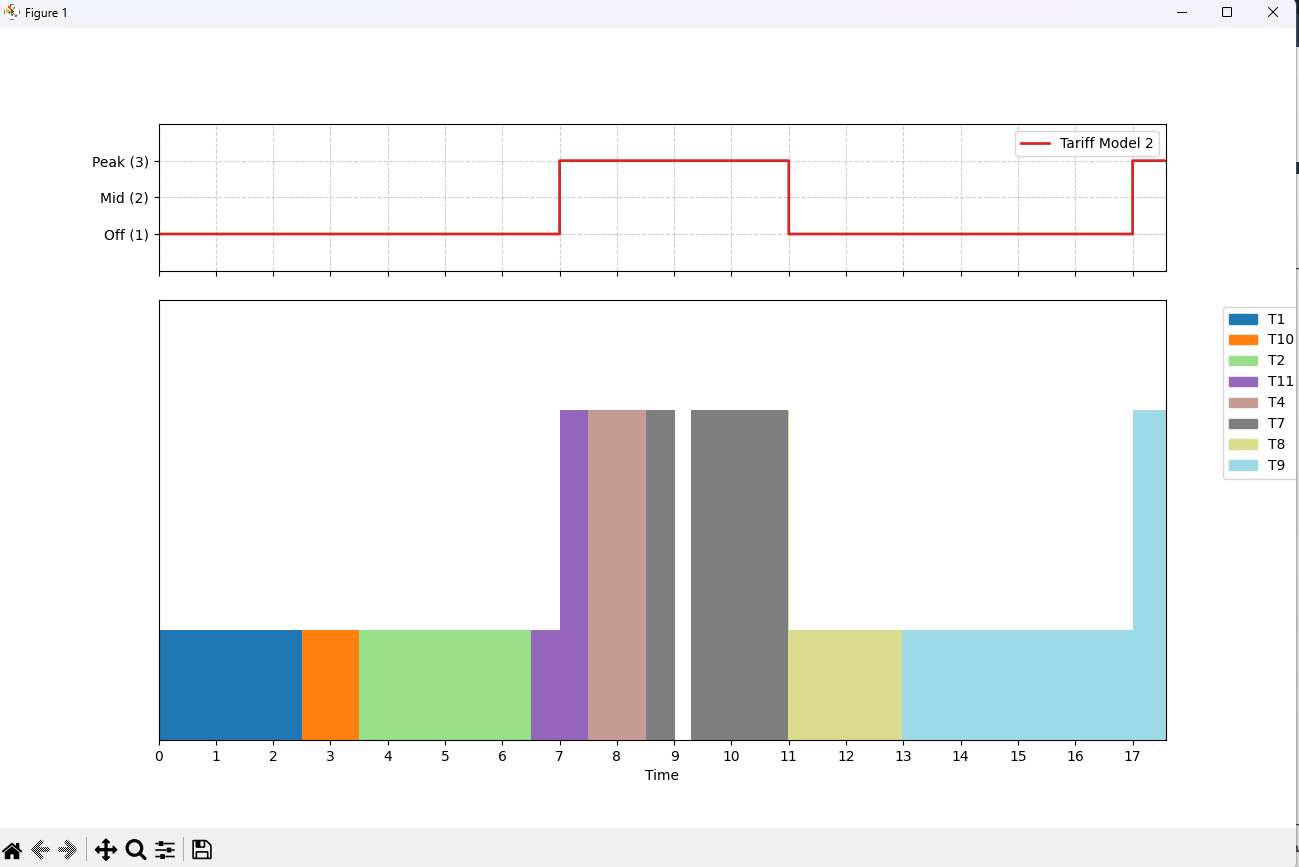
\includegraphics[width=0.92\textwidth]{image.png}
    \caption{Ordonnancement obtenu et signal tarifaire associé (Modèle Tariff 2)}
    \label{fig:gantt-tarif}
\end{figure}

\section{Synthèse et positionnement des approches}

\begin{itemize}
    \item \textbf{EDF glouton} : meilleure fiabilité temporelle, coût élevé
    \item \textbf{Horizon glissant} : meilleur compromis coût/efficacité dans un contexte dynamique
    \item \textbf{Programmation Dynamique} : référence optimale théorique (uniquement hors-ligne)
\end{itemize}

L’approche à horizon glissant apparaît comme la plus adaptée à un système réel soumis à des tarifications dynamiques et à des arrivées asynchrones de tâches.

\end{document}